\documentclass[11pt]{article}
\usepackage{amsmath}
\usepackage{amssymb}
\usepackage{graphicx}
\usepackage{nips15submit_e, times}
\usepackage[T1]{fontenc}

\title{Final Report: Semi-Supervised Learning of Pen-Based OCR.}
\author{Joshua Brakensiek, Jacob Imola, Sidhanth Mohanty}

\begin{document}

\maketitle

\begin{abstract}

  This report explores using semi-supervised learning to classify vector-based representations of handwritten digits. We describe related semi-supervised approaches such as transductive support vector machines (TSVMs), spectral graph transducers, and neural networks. We exposit our experimental results with these methods, and explore major takeaways of this project.

\end{abstract}



\newcommand{\Seq}{\operatorname{Seq}}

\section{Background}

Handwriting recognition is a classic machine learning problem. Generally, an image of a digit is inputted to an algorithm and classified. Instead of taking this approach, we used the sets,  ``Pen-Based Recognition of Handwritten Digits Data Set'' \cite{Alpaydin:1998} from the UCI Machine Learning Repository \cite{Lichman:2013}, which consist of pixel coordinates that the writers' pens took at certain time intervals. This data set, which has over 10,000 data points, consists entirely of drawings of the digits $0, \hdots, 9$. We seek to explore if adding the extra information of time while sacrificing some detail from the shape of the digits can produce a viable semi-supervised model.  We implement our learning algorithms in Python 2.7, using on the NumPy, SciPy, and Scikit-learn libraries (and possibly other libraries as we see fit). Our algorithms build off of SVMs and neural nets, both supervised models.

\section{Related Work}

The TSVM algorithm that we implemented requires that in the unlabeled
data, the number of data points classified is constrained to be
exactly equal to some parameter $num_+$. \cite{joachims2003transductive}
shows that this special kind of TSVM is equivalent to solving
a $s$-$t$ min cut problem, where the size of the partitions are fixed beforehand, and explores an algorithm called spectral graph transducer,
that does not require the sizes of the partitions to be fixed beforehand.

Closely related to the graph interpretation of semi-supervised SVMs
are methods intersecting at spectral graph theory and semi-supervised
learning like Laplacian SVMs and Manifold regularization
(see \cite{belkin2005manifold}). This method assume a distribution $P$
over $X\times \mathbb{R}$ from which labeled examples $(x,y)$ are drawn,
and assumes that the marginal distribution of $P$ on $X$, denoted $P_X$,
has the structure of a Riemannian manifold and uses this model
as a basis for a family of methods.

Another related semi-supervised learning technique that could
be applied to TSVMs is co-training, introduced in
\cite{blum1998combining}. This technique splits each unlabeled
example into multiple `views' (an example as specified in \cite{blum1998combining} would be how webpages can be partitioned into
the content on that page and content on other pages that link to it),
and two learning algorithms are trained on different views. Then,
the labels provided by the algorithms on previously unlabeled examples
are used to increase the labeled data available to the other
algorithm to train on.

\cite{joachims1999making} describes an algorithm called $SVM^{light}$,
which is faster than traditional algorithms for training
semi-supervised SVM that scales well with a large amount of
data, but sacrifices on accuracy.

\section{Methods}

\subsection{TSVM}

One TSVM method we use is an SVM with local search which was first described in \cite{Joachims:1999}, and we describe his algorithm briefly. Let $X = \{x_1, x_2, \ldots, x_k\}$ be the labeled training data, $Y = \{y_1, y_2, \ldots, y_k\}$ be the corresponding labels, $X^* = \{x^*_1, x^*_2, \ldots, x^*_n\}$ be the unlabeled training data, and $Y^* = \{y^*_1, y^*_2, \ldots, y^*_n\}$ be variables representing the unlabeled training data's labels. Recall that an SVM reduces to the following primal problem:

\begin{equation}\label{eq:1}
\arg\min_{w, b, \zeta} \frac{1}{2}w^Tw+C\sum_{i=1}^k\zeta_i
\end{equation}

\begin{align*}
\textrm{subject to}\quad \forall_{i=1}^k&: y_i(wx_i+b)\geq 1-\zeta_i \\
\forall_{i=1}^k&: \zeta_i>0
\end{align*}
Here, we use a more general version of an SVM:
\begin{equation}\label{eq:3}
\arg\min_{w, b, \zeta,\zeta^*} \frac{1}{2}w^Tw+C\sum_{i=1}^k\zeta_i+C^*_+\sum_{i=1}^n\zeta^*_i[y^*_i == 1]+C^*_-\sum_{i=1}^n\zeta^*_i[y^*_i == -1]
\end{equation}

\begin{align*}
\textrm{subject to}\quad \forall_{i=1}^k&: y_i(wx_i+b)\geq 1-\zeta_i \\
\forall_{i=1}^n&: y^*_i(wx^*_i+b)\geq 1-\zeta^*_i \\
\forall_{i=1}^k&: \zeta_i>0 \\
\forall_{i=1}^n&: \zeta^*_i>0
\end{align*}

To implement our TSVM, the user inputs constants $C$, the weight given to the labeled data, $C^*$, the weight given to the unlabeled data, $num_+$, which is the number of $Y^*$ that will be equal to 1, and $\epsilon$, which is a weight to be used later. First, a regular SVM is trained with $X$, $Y$, and $C$, using the objective function of (\ref{eq:1}). We take the $num_+$ most positive margin distances of $X^*$ and classify them as 1 in $Y^*$. Then, we initialize two weights, $C^*_- = \epsilon$ and $C^*_+ = \epsilon\frac{num_+}{n-num_+}$. Note that this gives more weight to whichever label, $+$ or $-$, should have more instances, and that both weights are small, representing that the accuracy of the unlabeled weights is not very high. Then, we call an SVM with the objective function of (\ref{eq:3}), using both $X$ and $X^*$ as our input data and $Y$ and $Y^*$ to be as our outputs. This new SVM may have two points, $x^*_i$ and $x^*_j$ in $X^*$, that have opposite labels yet are both misclassified by the SVM, or one is very misclassified and the other is classified correctly, but in the margin. In this case, we flip the labels of $x^*_i$ and $x^*_j$ because this preserve the number of positive $num_+$ examples and reduces the objective function of (\ref{eq:3}). We do this for as many points as possible, and then set $C^*_+ = \max\{2C^*_+, C^*_+\}$ and $C^*_- = \max\{2C^*_-, C^*_-\}$. This increases the importance of the unlabeled data because its label accuracy should be increasing. Then, we repeat the above procedure, training an SVM with the updated values of $C^*_+$, $C^*_-$, and $Y^*$, and repeating until $C^*_- = C^*_+ = C^*$.\par
To classify the digits, we trained ten one-vs-all TSVMs, one for each digit. To classify a new digit, we output whichever digit had the TSVM with the highest positive margin. We feel that the margin of the TSVM roughly corresponds with how confident the TSVM is. We also try error-correcting codes (Section \ref{codes}). We experiment with four kernels: polynomial, Gaussian, linear, and sigmoid.

\subsection{Semi-supervised Neural Network}

Another line of attack explored is implementing a semi-supervised deep neural net. The neural net we constructed in an adaptation the \emph{pseudo-label} algorithm due to \cite{Lee:2013}. Lee's algorithm consists of a unsupervised phase, a supervised phase, and a semi-supervised phase. The first phase ignores the labels entirely and trains an autoencoder to get a better representation of the data. The second phase uses the labeled data to train the full network using gradient descent and dropout. For the final phase, Lee uses the method of \emph{pseudo-labels} to utilize more fully the unlabeled data. In this method, during each round of gradient descent, the neural net is trained on both kinds of data. The labeled data is treated as normally. For the unlabeled data, a classification is chosen based on most most highly activated output unit for the unlabeled data point, and the accuracy of the neural network on that data point is measured from the inferred classification.

We implemented a modified version of Lee's algorithm. The neural network we use consists of four layers: the input nodes, the hidden layer, and the output nodes. There are 16 input nodes which encode the data in its original form. The autoencoder layer stores a better representation of the data. The hidden layer consists of 12 hidden units. The output layer consists of 26 units, 16 units which are trained as an autoencoder and 10 units which are trained for classification. Initially all the weights are set to small random values. During the first phase, we train the neural network only on the labeled data, attempting to minimize the sum of the squared error of the autoencoder and the classification units, where we weight the autoencoder three times as much as the classification units. We use 50 iterations for this stage. For the second phase, we train both the labeled and unlabeled data trying to minimize both the autoencoder and the classification units, where we use the pseudolabels for the unlabeled data to judge the classification accuracy. We also weight the autoencoder now four times as much instead of three times as much to emphasize the use of the unlabeled data to assist the autoencoder. This lasts for 250 iterations. In both phases, we use the backpropogation algorithm with momentum as described in the lecture. The gradient descent step size was steadily decreasing for the labeled data while it was steadly increasing for the labeled data.

\subsection{Error-correcting code for TSVM}
\label{codes}
A different approach to training binary TSVMs to classify digits is  to train many classifiers using different kinds of splits and aggregating the results with an error-correcting code to decide on a classification. This approach is inspired by the recent work of \cite{DBLP:journals/corr/BalcanDM15}.

In this approach, we associate each class (in our case, each class
is a digit) to a point in the space $\{-1,+1\}^k$
for some appropriately chosen $k$. We choose our points as codewords
of some error correcting code, which for our purposes means that the
representations of any 2 digits in this transformed space are
far apart: a digit would look something like $(-1,1,1,-1,-1,1)$.
A separate transductive SVM is trained on each entry in the tuple,
and classification is performed on a new datapoint $x$ by picking the
class that is least Hamming distance away from the classification
$(h_1(x),\ldots,h_k(x))$ where the $h_i$ are the separately trained
classifiers.

The representations of the digits we chose were the codewords of the
(7,4)-Hamming code \cite{macwilliams1977theory}. They have the property that any
any two codewords are Hamming distance 3 apart, and are robust up to
a single corruption. This means that if the class for digit 2 was
$(-1,1,-1,1,1)$ and the classifier on the fourth bit was incorrect
leading to $(-1,1,-1,-1,1)$, the algorithm would still correctly
classify the datapoint as digit 2.

A distinct advantage this might have over the one-vs-all
classifier is its robustness if one classifier makes a mistake.

\subsection{Autoencoder + TSVM}

[ACTUALLY DO THIS] An additional aspect we explored is trying different representations of our feature space (besides kernels). The different representation we tried is a compressed one using an autoencoder. We modified the neural network code mentioned above to produce to train an autoencoder on both the labeled and unlabeled training examples. Using the representation given by the hidden units in this autoencoder, we then trained a family of TSVMs to classify this data.

\subsection{Spectral Graph Transducer}
Another method we use is a semi-supervised version of $k$-Nearest Neighbors known as the Spectral Graph Transducer, as described in \cite{joachims2003transductive}. First, a similarity
graph is constructed where the vertices are the data points (both labeled
and unlabeled) and have edges weighted by some notion of similarity, like
distance in a metric space.
And under the 3 goals of achieving low training error, having the 
transductive algorithm match its inductive counterpart, and achieving
approximately the same expected ratio between positive and negative examples 
in both labeled and unlabeled data, \cite{joachims2003transductive}
reduces the problem of weighted $k$NN to approximating the unconstrained
ratio cut on the similarity graph.

Let $L^+$ denote the set of labeled positive examples, and let
$L^-$ denote the set of labeled negative examples.
The unconstrained ratio cut problem can be stated as follows.

\[\arg\max_{(G^+, G^-)}\frac{\mathrm{cut}(G^+,
G^-)}{\lvert G^+\rvert\lvert G^-\rvert}\]

\begin{align*}
\text{subject to }\quad x\in G^+\text{ if }x\in L^+\\
x\in G^-\text{ if }x\in L^-
\end{align*}

Here, $\mathrm{cut}(G^+, G^-)$ denotes the sum of weights of
edges between $G^+$ and $G^-$. As described in \cite{dhillon2001co}, the problem can be equivalently written as

\[\arg\min_{\vec{z}}\frac{\vec{z}^T L\vec{z}}{\vec{z}^T\vec{z}}\]
\[\text{subject to }\quad z_i\in\{\gamma_+,\gamma_-\}\]

where $L$ is the Laplacian matrix of the graph $G$,
$\gamma_+=\sqrt{\frac{\lvert L^-\rvert}{\lvert L^+\rvert}}$
and $\gamma_-=-\sqrt{\frac{\lvert L^+\rvert}{\lvert L^-\rvert}}$.
This problem, though NP-hard, can
be approximated well. The approximation arises in considering the real relaxation of the problem where one minimizes $\vec{z}^TL\vec{z}$
under the constraints that $\vec{z}^T1=0$ and $\vec{z}^T\vec{z}=n$,
for which the solution happens to be the second largest eigenvalue of
$L$.

Under the constraint that elements in $L^+$ must be in $G^+$
partition and elements in $L^-$ must be in $G^-$ partition,
the objective function we must minimize changes to
$\vec{z}^TL\vec{z}+c(\vec{z}-\vec{\gamma})^TC(\vec{z}-\vec{\gamma})$,
the original objective with an added quadratic penalty, with $c$
being the tradeoff parameter and $\vec{\gamma}$ being a vector
with dimension equal to the number of datapoints where $\gamma_i$
is $\gamma_+$ if the $i$-th datapoint is in $L^+$, $\gamma_-$
if the datapoint is in $L^-$ and 0 otherwise.

The algorithm for approximating the minimum of the objective is described
in \cite{joachims2003transductive}.


\section{Data, Experiments, and Results}

We have exclusively utilized the ``Pen-Based Recognition of Handwritten Digits Data Set'' from \cite{Alpaydin:1998}. We had previously considered supplementing with data from another We have also not yet incorporated the second data set from \cite{Llorens:2008}, but we decided not to incorporate this data since it is in a different format and it has more symbols such as Latin letters and Unicode characters and there are fewer samples per character.

The data presented in \cite{Alpaydin:1998} is a normalized time series of a user drawing a digit. Specifically, each input consisted of eight points in $[0, 100]^2$, representing the location of the pen at each step of drawing the digit. Often the originally collected data by the designers had more steps, but the data set was normalized to achieve uniformity of data while still preserving accuracy. The classifier $h$ we seek to train consists is thus a function from $[0, 100]^{16} \to \{0, 1, \hdots, 9\}$.  As the goal of this project is semi-supervised learning, we partitioned the data into three groups, labeled training data, unlabeled training data, and testing data. The data was already pre-divided into training and testing batches. We used random sampling to make some fraction of the data unlabeled. Our tests would use 0.5\%, 1\%, 5\%, 10\%, 20\%, and 50\% labeled data to understand the impact of more labeled data on our methods.

We tested the searching algorithm used in \cite{Joachims:1999} on this data set
with two different approaches.
In one approach, we trained 10 different TSVMs, one to distinguish one digit from the rest of the data (the approach we have been referring to as one-vs-all approach.
To classify a given test point, we found the signed distance from the point to the decision boundary of each TSVM and found the maximum.

The second approach we used was the one based on error correcting codes,
described in section 3.3.

A baseline we had earlier was one-vs-all using a linear kernel,
which performed at 88\% accuracy on 20\% labeled data. Using the polynomial
kernel $(x_i\cdot x_j + 3)^5$
brought the test accuracy up to 96\%, and using a Gaussian kernel
where the kernel function was of the form $e^{-0.8\|x_i-x_j\|^2}$
earned a test accuracy of 97\%. The error correcting codes technique
performed slightly worse, with a test accuracy of 82\% on the linear kernel,
95\% on the polynomial kernel and 96\% on the Gaussian kernel.

We found it surprising that a straightforward one-vs-all
approach performed better than the error-correcting codes approach,
since the latter approach was engineered to be robust to classification
error.

An approach that might have yielded better results is
using a code with greater redundancy such as the Hadamard
code \cite{macwilliams1977theory}.
This way, the algorithm would be robust to more errors on separate entries
of the tuple.
Additionally, the way the codewords were assigned to digits was arbitrary
and a more careful assignment that put more distant codewords on
similar digits (like 1 and 7, or 4 and 9) would decrease the chance
of the algorithm confusing similar digits.

Our implementation of one-vs-all took the margin of classification
into account (in particular, it returned the class with maximum margin of
classification), but our approach using error correcting codes does not do that,
which might be a reason one-vs-all slightly 
outperforms error correction. This may suggest that having a high margin
on a single classifier is more indicative of the correct class than
the number of classifiers that correctly classified a point.

The neural network did about as well as the baseline TSVM approach. Also, it is not clear that the unlabeled data assisted much except perhaps prevent overfitting.

\begin{table}[]
  \centering
  \caption{This table represents the accuracy of our TSVM classification using
  the error correcting codes approach and the Gaussian kernel
 with 20\% labeled data. The overall accuracy is 96.4\%. Each column represents the actual digit which was drawn, and each row represents the label given by our algorithm. For example, there were several digits with multiple instances
  incorrectly labeled as 1's, whose codewords were relatively close to the
  codeword of 1.}
  \label{my-table}
  \vspace{.3in}
  \begin{tabular}{l|llllllllll}
    & 0 & 1 & 2 & 3 & 4 & 5 & 6 & 7 & 8 & 9\\\hline
    0 &351 & 0   & 0   & 0   & 0   & 0   & 0   & 0   & 3   & 0   \\
    1 &10   & 339 & 1  & 1   & 1   & 12   & 1   & 15  & 5   & 12  \\
    2 & 0   & 19  & 362 & 0   & 0   & 0   & 0   & 3   & 0   & 0   \\
    3 & 0   & 0   & 0   & 330 & 0   & 5  & 0   & 0   & 0   & 0   \\
    4 & 0   & 1   & 0   & 0   & 351 & 0   & 0   & 0  & 0   & 0   \\
    5 & 0   & 0  & 0   & 0   & 9  & 313 & 1   & 0   & 1  & 0  \\
    6 & 8   & 1   & 0   & 0   & 6   & 3   & 334 & 1   & 0   & 0   \\
    7 & 0   & 5   & 1   & 3   & 3   & 5   & 0   & 345 & 0   & 4   \\
    8 & 2  & 0   & 0   & 0   & 0   & 0   & 0   & 0   & 330 & 1   \\
    9 & 0   & 0   & 0   & 2   & 0  & 0  & 0   & 2   & 0   & 319
  \end{tabular}
  \end{table}

Finally, we produced a noticeable relationship between percent of labeled data and classification accuracy [REMAKE PLOT FOR GAUSSIAN KERNEL ON
one-vs-all ON 20\% LABELED DATA AND (POSSIBLY) ADD CONFUSION MATRIX
FOR one-vs-all] \par

%[Insert graph of classification accuracy vs percent of labeled data]\par
\begin{figure}
  \centering
  \caption{The following graph plots accuracy of our TSVM classifier based on the fraction of labeled data. We ran the TSVM on 0.5\%, 1\%, 2\%, 5\%, 10\%, 20\%, 50\%, and 80\% labeled data. Note as the amount of labeled data increases, it becomes marginally less useful.}
  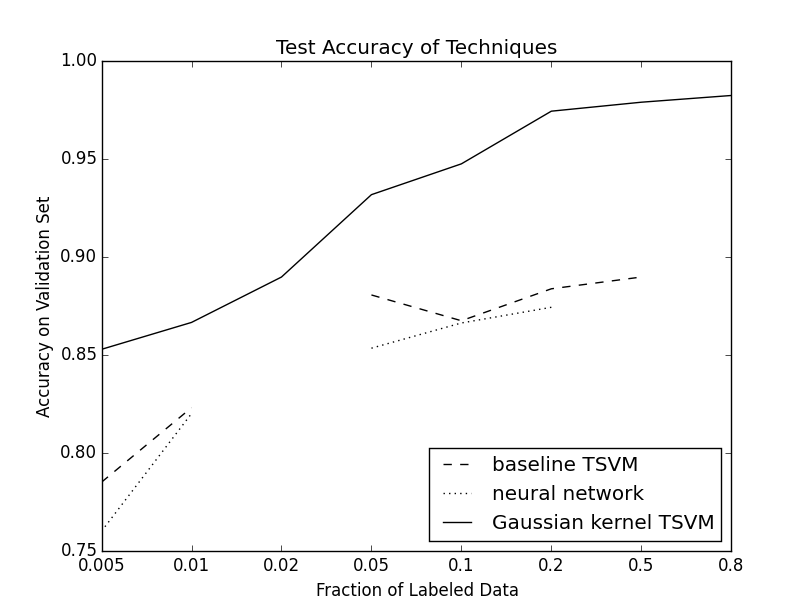
\includegraphics[width=5in]{figure_1.png}
\end{figure}

%[Insert comments about digits that the TSVM often mistook for another]

As can be seen in the confusion matrix of the error correcting codes,
5, 7 and 9 were misclassified by 1's and the codewords for
these digits that we picked had Hamming distance 3 away from 1, which
explains why the confusion was likely.


\section{Future Plans}

[INTEGRATE THESE THINGS]

Another area of exploration is trying different kernels for the TSVM, perhaps something more complex than a linear kernel and not as advanced as a Gaussian kernel. Doing feature selection could help us find a good kernel. For example, we could change the algorithm of \cite{Joachims:1999} by not enforcing exactly $num_+$ examples to be classified as +1. Another approach would be to use the Graph kernel methods of \cite{smola2003kernels}. We would also like to try different values for the parameters in the algorithm.

\section{Conclusions and Lessons Learned}

From completing this project, we have learned a few important ideas about semisupervised learning. 

We learned the notion of the bandwidth of a kernel, that is,
how certain constant parameters can make a big difference in how well
a kernel SVM performs. For example, when we initially tried the
Gaussian kernel, it performed poorly since the value
$c$ in $e^{-c\|x_i-x_j\|^2}$ was fairly large.
On tuning $c$ however, the performance was much better. In particular,
before tuning $c$, the decision boundary looked like a collection of
small balls around the datapoints.

When implementing the neural networks, we learned that it is quite difficult to use the unlabeled data without falling into a confirmation bias. Using the autoencoder was quite useful in that regard. It is not clear how much the unlabeled data assisted in finding a better fit. Furthermore, more experimentation could have been done to determine the correct momentum and step sizes.

\bibliographystyle{alpha}
\bibliography{final}

\end{document}
